% enable this to activate the version for PRINT
% disable this to make the pdf symmetric and without white pages
% => asymmetric alternating left/right margins
% \newcommand*{\printversion}{}%

%% | ---------------- document meta information --------------- |

\newcommand{\Author}{Jakub Pelc}
\newcommand{\Department}{Department of Cybernetics}
\newcommand{\Supervisor}{Ing. Vojtěch Vrba}
%\newcommand{\SupervisorSpecialist}{Ing. My Specialist, Ph.D.}
\newcommand{\Programme}{Open Informatics}
\newcommand{\Field}{Artificial Intelligence and Computer Science}
\newcommand{\Title}{Analysis of an influnce of a modulated light source frequency \\[0.5em] and distance on an event-based camera response}
\newcommand{\Keywords}{Unmanned Aerial Vehicles, Event Cameras}
\newcommand{\KlicovaSlova}{Bezpilotní Prostředky, Eventové Kamery}
\newcommand{\Year}{2025}
\newcommand{\Month}{January}
\newcommand{\Date}{\Month~\Year}
\newcommand{\Location}{Prague}

%% | ---------------------- configuration --------------------- |

% most of the configuration stuff happens here
%!TEX root = ../main.tex

%% | ----------------------- page setup ----------------------- |

% define documentclass based on the print/screen version of the document
\pdfoutput=1
\ifdefined\printversion
  \documentclass[a4paper,11pt,twoside,openright]{book}
\else
  \documentclass[a4paper,11pt,twoside,openany]{book}
\fi

% define how "clearpage" works with the print/screen version of the document
\newcommand{\conditionalClearPage}{
  \ifdefined\printversion
    \cleardoublepage
  \else
    \clearpage
  \fi
}

%% | ----------------- commonly used packages ----------------- |

\usepackage[english]{babel}
\usepackage[utf8]{inputenc}
\usepackage{csquotes}
\usepackage{amsmath,amsfonts,amssymb,bm}
\usepackage{nicefrac}
\usepackage{algorithm,algpseudocode}
\usepackage[title,titletoc]{appendix}
\usepackage{latexsym}
\usepackage{a4wide}
\usepackage{color}
\usepackage{indentfirst}
\usepackage{graphicx}
\usepackage{fancyhdr,lastpage}
\usepackage{longtable}
\usepackage{pifont}
\usepackage{makeidx}
\usepackage{multirow}
\usepackage{dcolumn}
\usepackage{epstopdf}
\usepackage{url}
\usepackage{listings}
\usepackage{relsize}
\usepackage{pdfpages}
\usepackage{url}
\usepackage{lipsum}
\usepackage{isotope}
\usepackage{verbatim}
\usepackage{xcolor}
\usepackage{tcolorbox}
\usepackage[colorlinks]{hyperref}
\usepackage{multicol}
\usepackage{subfig}
\usepackage[export]{adjustbox}

% print version has different margins to accommodate the spine of the book
% do not move this around, or it stops working
\ifdefined\printversion
  \usepackage[a4paper,margin=3.2cm,inner=3.4cm,outer=2.0cm]{geometry}
\else
  \usepackage[a4paper,margin=3.2cm,inner=2.7cm,outer=2.7cm]{geometry}
\fi

\hyphenation{}

%% | --------------------- custom commands -------------------- |

\definecolor{cvutblue}{cmyk}{1, 0.43, 0, 0}

% set itemize: bullets type and color
\renewcommand{\labelitemi}{\textcolor{cvutblue}{\raisebox{.45ex}{\rule{.8ex}{.8ex}}}}
\renewcommand{\labelitemii}{\textcolor{cvutblue}{\raisebox{.45ex}{\rule{.8ex}{.8ex}}}}
\renewcommand{\labelitemiii}{\textcolor{cvutblue}{\raisebox{.45ex}{\rule{.8ex}{.8ex}}}}
\renewcommand{\labelitemiv}{\textcolor{cvutblue}{\raisebox{.45ex}{\rule{.8ex}{.8ex}}}}


%% | ---------------------- abbreviations --------------------- |

\usepackage[printonlyused]{acronym}

% use to change margins around abbreviations block
\def\changemargin#1#2{\list{}{\rightmargin#2\leftmargin#1}\item[]}
\let\endchangemargin=\endlist

%% | -------------------- hyper links setup ------------------- |
\hypersetup{
  linkcolor=black,
  anchorcolor=black,
  citecolor=cvutblue,
  filecolor=black,
  menucolor=black,
  runcolor=black,
  urlcolor=cvutblue
}


%% | -------------------------- tikz -------------------------- |

\usepackage{tikz}
\usepackage{pgfplots}
\pgfplotsset{compat=1.14}
\usetikzlibrary{backgrounds,arrows,automata,shapes,positioning,calc,through,spy,shapes,shapes.geometric,shapes.multipart,fit,patterns,fadings}
\pgfdeclarelayer{background}
\pgfdeclarelayer{foreground}
\pgfsetlayers{background,main,foreground}

%% | ------------ siunitx for units of measurements ----------- |

\usepackage{siunitx}
\DeclareSIUnit \parsec {pc}
\DeclareSIUnit \electronvolt {eV}
\DeclareSIUnit \pixel {px}
\DeclareSIUnit \arcmin {arcmin}
\DeclareSIUnit \erg {erg}
\DeclareSIUnit \joul {J}

%% | --------------- change formatting of lists --------------- |

\usepackage{enumitem}
\setlist{nosep}

\renewcommand{\labelenumi}{(\roman{enumi})}

%% | -------------------- table of contents ------------------- |

\usepackage[subfigure]{tocloft}

\tocloftpagestyle{plain}

%% | ----------------- formatting of a chapter ---------------- |

\usepackage{titlesec}

\titleformat{\chapter}[hang]{}{\color{cvutblue}\rule[-0.03cm]{0.50cm}{0.50cm}}{3.2\parskip}{\normalfont\bfseries\LARGE\thechapter\hspace{0.5cm}}
\titlespacing*{\chapter}{0pt}{-1em}{1.5em}

%% | ----------------- formatting of a section ---------------- |

\titleformat{\section}[hang]{}{\hspace{0.11cm}\color{cvutblue}\rule[-0.02cm]{0.30cm}{0.30cm}}{3.7\parskip}{\normalfont\bfseries\large\thesection\hspace{0.5cm}}
\titlespacing*{\section}{0pt}{1em}{0.5em}

\titleformat{name=\section,numberless}[block]
{\normalfont\large\bfseries}{}{0pt}{\large}
% {?}{before}{after}
\titlespacing*{name=\section,numberless}{0pt}{-1em}{2em}

%% | --------------- formatting of a subsection --------------- |

\titleformat{\subsection}[hang]{}{\hspace{0.16cm}\color{cvutblue}\rule[0.03cm]{0.20cm}{0.20cm}}{4.0\parskip}{\normalfont\bfseries\normalsize}
\titlespacing*{\subsection}{0pt}{1em}{0.5em}



%% | ------------------------ biblatex ------------------------ |

\usepackage[backend=bibtex,defernumbers=true,style=ieee,sorting=ydnt,sortcites=true]{biblatex}

% define the source file with bibliography
\addbibresource{main.bib}

\renewcommand*{\bibfont}{\Font}

% add suffix "a" to publications containing the keyword "mine"
% add suffix "c" to publications containing the keyword "mine" && "core"
\DeclareFieldFormat{labelnumber}{%
  \ifkeyword{mine}
    {\ifkeyword{core}
      {{\number\numexpr#1}c}%
      {{\number\numexpr#1}a}%
    }%
    {#1}%
}

\DeclareCiteCommand{\tabcite}%[\mkbibbrackets]
  {\usebibmacro{cite:init}%
   \usebibmacro{prenote}}
  {\usebibmacro{citeindex}%
   \usebibmacro{cite:comp}}
  {}
  {\usebibmacro{cite:dump}%
   \usebibmacro{postnote}}

% define fullciteinbox command
\definecolor{light-gray}{gray}{0.95}
\newcommand{\fullciteinbox}[2]{%

\DeclareCiteCommand{\fullcite}
{\usebibmacro{prenote}}
{\clearfield{addendum}%
  \usedriver
  {\defcounter{minnames}{6}%
  \defcounter{maxnames}{6}}
{\thefield{entrytype}}}
{\multicitedelim}
{\usebibmacro{postnote}}

\begin{tcolorbox}[opacityfill=0.05,width=\textwidth,colback={cvutblue},colframe={cvutblue},title={}]%
\ifx&#2&
\else
  \textbf{#2}:\\\\
\fi
\begin{minipage}[t]{0.07\linewidth}%
\raggedright%
\cite{#1}%
\end{minipage}%
\begin{minipage}[t]{0.93\linewidth}%
\fullcite{#1}%
\end{minipage}%
\end{tcolorbox}%
%}%
\vspace{-0.3em}
}%

% change the bibliography font style
% does not compile without this
\let\bibfont\small

% this is used to print citations of author's work
\defbibenvironment{mycitations}
{\itemize}
{\enditemize}
{\item}

%% | ---------------------- custom macros --------------------- |

\newcommand{\strong}[1]{\textbf{#1}}
\newcommand{\coord}[1]{\textbf{#1}}
\newcommand{\norm}[1]{\left\lvert#1\right\rvert}
\newcommand{\m}[1]{\ensuremath{\mathbf{#1}}}
\newcommand\numberthis{\addtocounter{equation}{1}\tag{\theequation}}
\newcommand{\add}[1]{{\color{green} {#1}}}
\newcommand{\todo}[1]{{\color{red} TODO {#1}}}
\newcommand{\updated}[1]{{\color{blue} {#1}}}
\newcommand{\real}{\mathbb{R}}
\newcommand{\red}[1]{{\color{red} #1}}
\newcommand{\minus}{\scalebox{0.75}[1.0]{$-$}}
\newcommand{\plus}{\scalebox{0.8}[0.8]{$+$}}
\newcommand{\figvspace}{\vspace{-1em}}

% referencing
\newcommand{\reffig}[1]{Fig.~\ref{#1}}
\newcommand{\reflst}[1]{Lst.~\ref{#1}}
\newcommand{\refalg}[1]{Alg.~\ref{#1}}
\newcommand{\refsec}[1]{Sec.~\ref{#1}}
\newcommand{\reftab}[1]{Table~\ref{#1}}
\newcommand{\refeq}[1]{\eqref{#1}}

\newcommand{\refchap}[1]{chapter~\ref{#1}}

%% | ----------------- listings - showing code ---------------- |

\usepackage{listings}     
\usepackage{lstautogobble}  % Fix relative indenting
\usepackage{color}          % Code coloring
\usepackage{zi4}            % Nice font

\definecolor{bluekeywords}{rgb}{0.13, 0.13, 1}
\definecolor{greencomments}{rgb}{0, 0.5, 0}
\definecolor{redstrings}{rgb}{0.9, 0, 0}
\definecolor{graynumbers}{rgb}{0.5, 0.5, 0.5}

\usepackage{listings}
\lstset{
    autogobble,
    columns=fullflexible,
    showspaces=false,
    showtabs=false,
    breaklines=true,
    showstringspaces=false,
    breakatwhitespace=true,
    escapeinside={(*@}{@*)},
    commentstyle=\color{greencomments},
    keywordstyle=\color{bluekeywords},
    stringstyle=\color{redstrings},
    numberstyle=\color{graynumbers},
    basicstyle=\ttfamily\footnotesize,
    frame=l,
    framesep=12pt,
    xleftmargin=12pt,
    tabsize=4,
    captionpos=b
}

%% | -------------------- layout parameters ------------------- |

% no indent, free space between paragraphs
\setlength{\parindent}{1cm}
\setlength{\parskip}{1ex plus 0.5ex minus 0.2ex}

% offsets the head down
\setlength{\headheight}{18pt}

% foot line
\renewcommand{\footrulewidth}{0.4pt}

%% | -------------- define the 'full' page style -------------- |

\fancypagestyle{full}{%

  % clear the default layout
  \fancyhead{}
  \fancyfoot{}

  % page header
  \fancyhead[LO]{\leftmark}
  \fancyhead[RE]{\rightmark}
  \fancyhead[LE,RO]{\thepage/\pageref{LastPage}}

  % page footer
  \fancyfoot[L]{CTU in Prague}
  \fancyfoot[R]{\Department}
  \fancyfoot[C]{}
}

%% | -------------- define the 'plain' page style ------------- |

\fancypagestyle{plain}{%

  % clear the default layout
  \fancyhead{}
  \fancyfoot{}

  % page header
  \fancyhead[LE,RO]{\thepage}
}

%% | -------------- Adjust style of chapter names ------------- |

\renewcommand{\chaptermark}[1]{\markboth{\MakeUppercase{\thechapter.\ #1}}{}}

%% | -------- European layout, no extra space after '.' ------- |

\frenchspacing

%% | ----------- adjust the style of the first page ----------- |

\makeatletter
\renewcommand\chapter{\if@openright\cleardoublepage\else\clearpage\fi
                    \thispagestyle{full}% original style: plain
                    \global\@topnum\z@
                    \@afterindentfalse
                    \secdef\@chapter\@schapter}
\makeatother


%% | ---------------------- the contents ---------------------- |

\begin{document}

% this will prevent unwanted line overflows
% http://latexref.xyz/_005cfussy-_0026-_005csloppy.html
\sloppy

\pagenumbering{roman}

%% --------------------------------------------------------------
%% |                         Title page                         |
%% --------------------------------------------------------------

%!TEX root = ../main.tex

\begin{titlepage}
  \begin{center}

    \textsc{\Large Czech Technical University in Prague}\\[1em]
    \textsc{\large Faculty of Electrical Engineering\\
    \Department\\
    Multi-robot Systems\\[3em]
    }
    
\includegraphics[height=4.1cm]{fig/ctu_lion.pdf}\\[3em]

    \textbf{\textsc{\Large \Title}}\\[2em]

    \textbf{\Large B4BPROJ6 - Semestral project}\\[6em]

    \textbf{\huge \Author}\\[6em]

    {\large \Location, \Date}\\[3em]

    Study programme: \Programme\\
    Branch of study: \Field\\[4em]

    \textbf{Supervisor: \Supervisor}\\

    \vspace{2pt}

  \end{center}
\end{titlepage}


% set up the page style for the "intro" pages
\pagestyle{plain}

%% --------------------------------------------------------------
%% |                       Acknowledgments                      |
%% --------------------------------------------------------------

%\conditionalClearPage

%%!TEX root = ../main.tex

\section*{Acknowledgments}

Firstly, I would like to express my gratitude to my supervisor.

\vspace{2.5cm}


%% --------------------------------------------------------------
%% |                         Assignment                         |
%% --------------------------------------------------------------

%\conditionalClearPage

%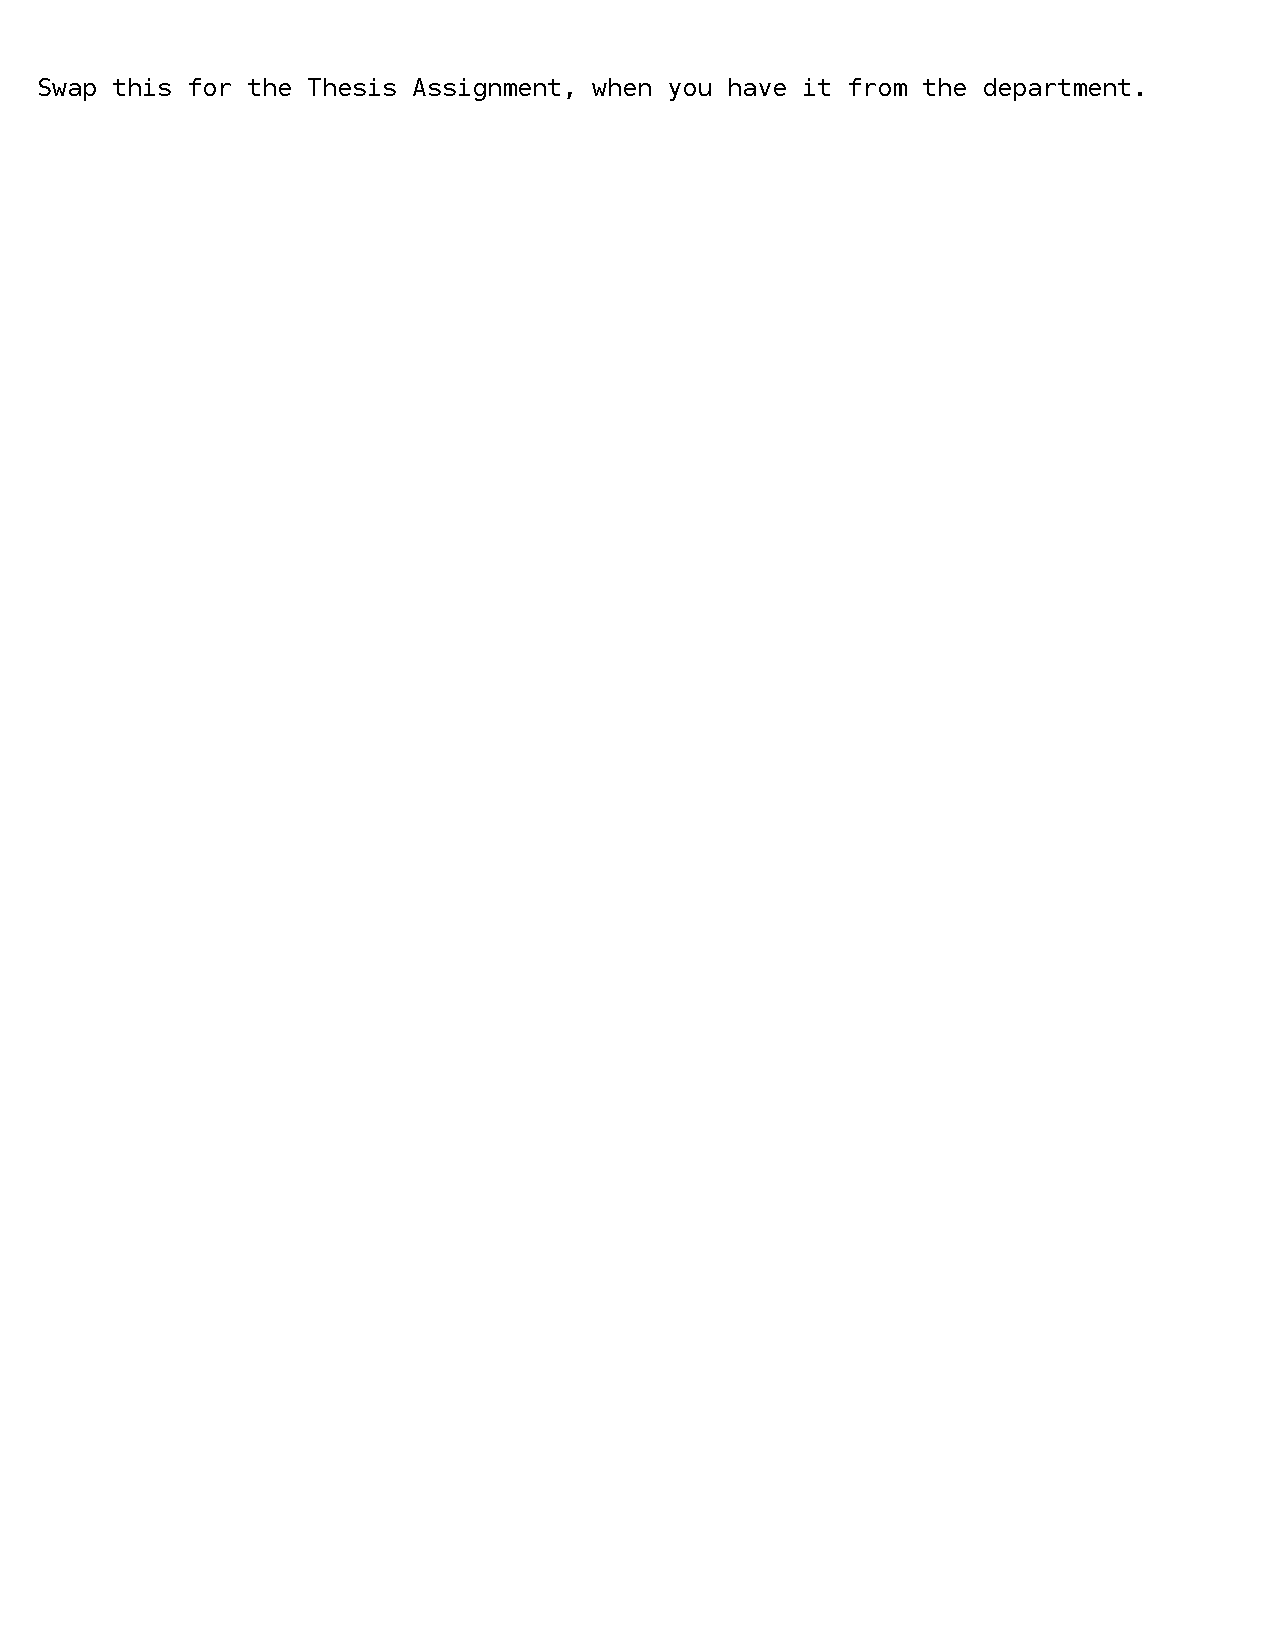
\includepdf{src/assignment.pdf}

%% --------------------------------------------------------------
%% |                         Declaration                        |
%% --------------------------------------------------------------

%\conditionalClearPage

%~\vfill{}

\section*{Declaration}
%\section*{Prohlášení autora práce}

I declare that presented work was developed independently, and that I have listed all sources of information used within, in accordance with the Methodical instructions for ob-serving ethical principles in preparation of university theses.
% Prohlašuji, že jsem předloženou práci vypracoval samostatně a že jsem uvedl veškeré použité informační zdroje v souladu s Metodickým pokynem o dodržování etických principů při přípravě vysokoškolských závěrečných prací.

\vspace{1.5cm}
~\\

Date .............................\hfill{}...............................................
% Dne.............................\hfill{}...............................................

\hfill{}~~~~~~~~~~~~~~~

\newpage{}


%% --------------------------------------------------------------
%% |                          Abstracts                         |
%% --------------------------------------------------------------

%\conditionalClearPage

%%!TEX root = ../main.tex

\begin{changemargin}{0.8cm}{0.8cm}

~\vfill{}

\section*{Abstract}
\vskip 0.5em

The study of autonomous \acp{UAV} has become a prominent sub-field of mobile robotics.

\vskip 1em

{\bf Keywords} \Keywords

\vskip 2.5cm

\end{changemargin}


%\conditionalClearPage

%%!TEX root = ../main.tex

\begin{changemargin}{0.8cm}{0.8cm}

~\vfill{}

\section*{Abstrakt}
\vskip 0.5em

\sloppy
Výzkum na poli autonomních bezpilotních prostředků (UAV) se stal významným oborem mobilní robotiky.

\vskip 1em

{\bf Klíčová slova} \KlicovaSlova

\vskip 2.5cm

\end{changemargin}


%% --------------------------------------------------------------
%% |                        Abbreviations                       |
%% --------------------------------------------------------------

\conditionalClearPage

\begin{changemargin}{0.8cm}{0.8cm}

~\vfill{}

\section*{Abbreviations}

% this will print only the used abbreviations
%!TEX root = ../main.tex

\begin{acronym}
  \acro{API}[API]{Application Programming Interface}
  \acro{CTU}[CTU]{Czech Technical University}
  \acro{DOF}[DOF]{degree-of-freedom}
  \acro{DVS}[DVS]{Dynamic Vision Sensor}
  \acro{FOV}[FOV]{Field of View}
  \acro{GNSS}[GNSS]{Global Navigation Satellite System}
  \acro{GPS}[GPS]{Global Positioning System}
  \acro{IMU}[IMU]{Inertial Measurement Unit}
  \acro{LED}[LED]{Light-Emitting Diode}
  \acro{LKF}[LKF]{Linear Kalman Filter}
  \acro{LTI}[LTI]{Linear time-invariant}
  \acro{LiDAR}[LiDAR]{Light Detection and Ranging}
  \acro{MAV}[MAV]{Micro Aerial Vehicle}
  \acro{MPC}[MPC]{Model Predictive Control}
  \acro{MRS}[MRS]{Multi-robot Systems Group}
  \acro{ROI}[ROI]{Region of Interest}
  \acro{ROS}[ROS]{Robot Operating System}
  \acro{RSSR}[RSSR]{Received Signal Strength Ratio}
  \acro{RTK}[RTK]{Real-time Kinematics}
  \acro{SLAM}[SLAM]{Simultaneous Localization And Mapping}
  \acro{UAV}[UAV]{Unmanned Aerial Vehicle}
  \acro{UGV}[UGV]{Unmanned Ground Vehicle}
  \acro{UKF}[UKF]{Unscented Kalman Filter}
  \acro{VLC}[VLC]{Visible Light Communication}
\end{acronym}


\vskip 2.5cm

\end{changemargin}

\conditionalClearPage

%% --------------------------------------------------------------
%% |                      Table of contents                     |
%% --------------------------------------------------------------

\tableofcontents

\conditionalClearPage

% set up the full page style with normal page numbering
\pagestyle{full}
\pagenumbering{arabic}

%% --------------------------------------------------------------
%% |                        introduction                        |
%% --------------------------------------------------------------

%!TEX root = ../main.tex

\chapter{Introduction\label{chap:introduction}}

Event based cameras, in contrast to traditional frame based cameras, do not capture still frames but rather
provide an asynchronous and independent stream of intensity changes on individual pixels.
Each pixel memorizes the last intensity value and sends an event when the intensity changes above a certain threshold.

Event cameras circumvent many common issues found in traditional frame-based cameras, such as motion blur caused
by fast-moving objects. They offer significant advantages, including a high dynamic range, low latency,
and energy efficiency.
This makes them perfect for the application of agile robotics,
where the fast response time is crucial (especially in UAV swarming situations). With their sub-millisecond response time,
event cameras can provide a significant advantage over traditional cameras in these applications.
However, they also come with some drawbacks, such as the need for a different approach to
data processing and the higher cost of the camera units themselves. \cite{gallego22event}


The event data stream is represented by tuples of $\begin{bmatrix} x & y & p & t \end{bmatrix}$, $\begin{bmatrix} x & y \end{bmatrix}$ are the pixel coordinates, $t$ is the time of
intensity change and $p$ is the polarity of the change - the increase or decrease of light intensity. Images can be
reconstructed from the event stream by integrating the events over time, doing so makes the usage of normal vision 
algorithms possible, but it also goes against the main advantage of the event cameras - the low latency.

\section{Related works}

This section should contain related state-of-the-art works and their relation to the author's work.

\section{Contributions}

This section should describe the author's contributions to the field of research.

\section{Mathematical notation}

It is a good practice to define basic mathematical notation in the introduction.
See \reftab{tab:mathematical_notation} for an example.

\begin{table*}[!h]
  \scriptsize
  \centering
  \noindent\rule{\textwidth}{0.5pt}
  \begin{tabular}{lll}
    $\mathbf{x}$, $\bm{\alpha}$ & vector, pseudo-vector, or tuple\\
    $\mathbf{\hat{x}}$, $\bm{\hat{\omega}}$& unit vector or unit pseudo-vector\\
    $\mathbf{\hat{e}}_1, \mathbf{\hat{e}}_2, \mathbf{\hat{e}}_3$ & elements of the \emph{standard basis} \\
    $\mathbf{X}, \bm{\Omega}$ & matrix \\
    $\mathbf{I}$ & identity matrix \\
    $x = \mathbf{a}^\intercal\mathbf{b}$ & inner product of $\mathbf{a}$, $\mathbf{b}$ $\in \mathbb{R}^3$\\
    $\mathbf{x} = \mathbf{a}\times\mathbf{b}$ & cross product of $\mathbf{a}$, $\mathbf{b}$ $\in \mathbb{R}^3$\\
    $\mathbf{x} = \mathbf{a}\circ\mathbf{b}$ & element-wise product of $\mathbf{a}$, $\mathbf{b}$ $\in \mathbb{R}^3$ \\
    $\mathbf{x}_{(n)}$ = $\mathbf{x}^\intercal\mathbf{\hat{e}}_n$ & $\mathrm{n}^{\mathrm{th}}$ vector element (row), $\mathbf{x}, \mathbf{e} \in \mathbb{R}^3$\\
    $\mathbf{X}_{(a,b)}$ & matrix element, (row, column)\\
    $x_{d}$ & $x_d$ is \emph{desired}, a reference\\
    $\dot{x}, \ddot{x}, \dot{\ddot{x}}$, $\ddot{\ddot{x}}$ & ${1^{\mathrm{st}}}$, ${2^{\mathrm{nd}}}$, ${3^{\mathrm{rd}}}$, and ${4^{\mathrm{th}}}$ time derivative of $x$\\
    $x_{[n]}$ & $x$ at the sample $n$ \\
    $\mathbf{A}, \mathbf{B}, \mathbf{x}$ & LTI system matrix, input matrix and input vector\\
    \emph{SO(3)} & 3D special orthogonal group of rotations\\
    \emph{SE(3)} & \emph{SO(3)}~$\times~\mathbb{R}^3$, special Euclidean group\\
  \end{tabular}
  \noindent\rule{\textwidth}{0.5pt}
  \caption{Mathematical notation, nomenclature and notable symbols.}
  \label{tab:mathematical_notation}
\end{table*}


%!TEX root = ../main.tex

\chapter{Measurements\label{chap:measurements}}

\section{Equipment}

The event based camera used in this work is the model EVK4\footnote{Prophesee EVK4 website: \url{https://www.prophesee.ai/event-camera-evk4/}.}, manufactured by Prophesee. The camera has a resolution of 
$1280 \times 720$ pixels, with maximum frame rate equivalent of 10k fps and a dynamic range of 120 dB.
A fish eye lens with an inbuilt UV filter was used during the measurements to target the specific wavelength of the LEDs
that are used on the UAVs. The camera is shown on \reffig{fig:evk4}. 

% \begin{figure}[htbp]
%   \centering
%   \subfloat[EVK4 event-based camera.] {
%     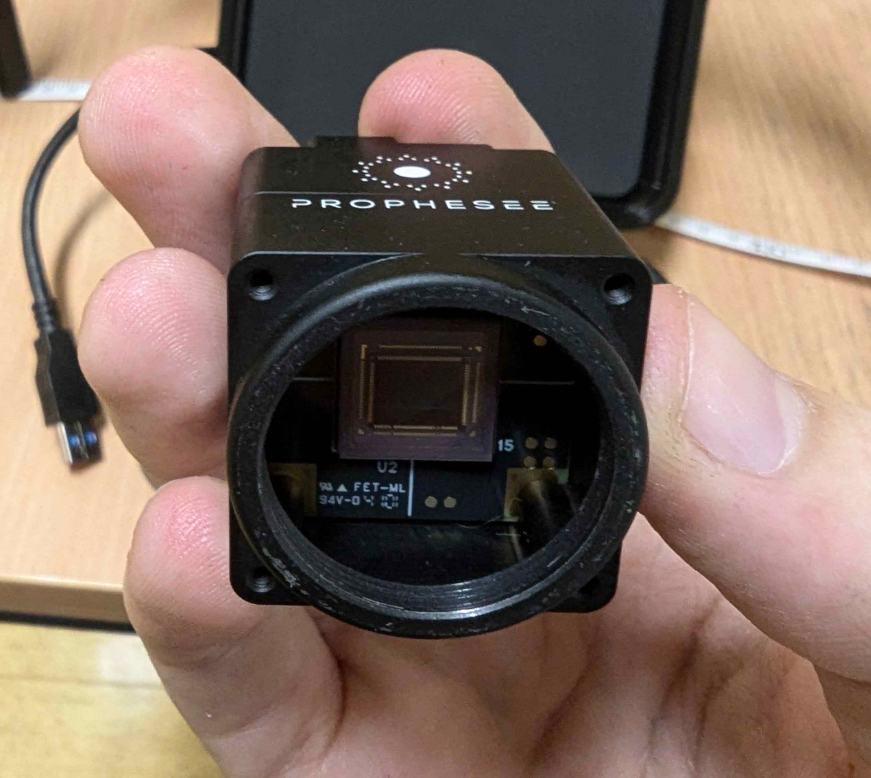
\includegraphics[width=0.3\textwidth]{./fig/photos/evk4.png}
%     \label{fig:evk4_1}
%   }
%   \subfloat[EVK4 event-based camera with a fish eye lens.] {
%     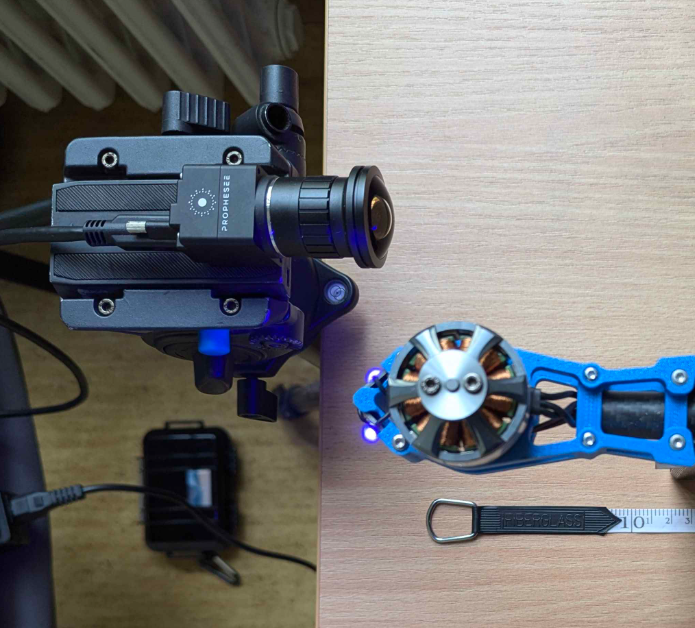
\includegraphics[width=0.3\textwidth]{./fig/photos/lens.png}
%     \label{fig:evk4_2}
%   }
%   \caption{
% The event based camera EVK4 from Prophesee, on \reffig{fig:evk4_1}, with a fish eye lens on \reffig{fig:evk4_2}.
% }
%   \label{fig:evk4}
% \end{figure}

\begin{figure}[htbp]
	\centering
	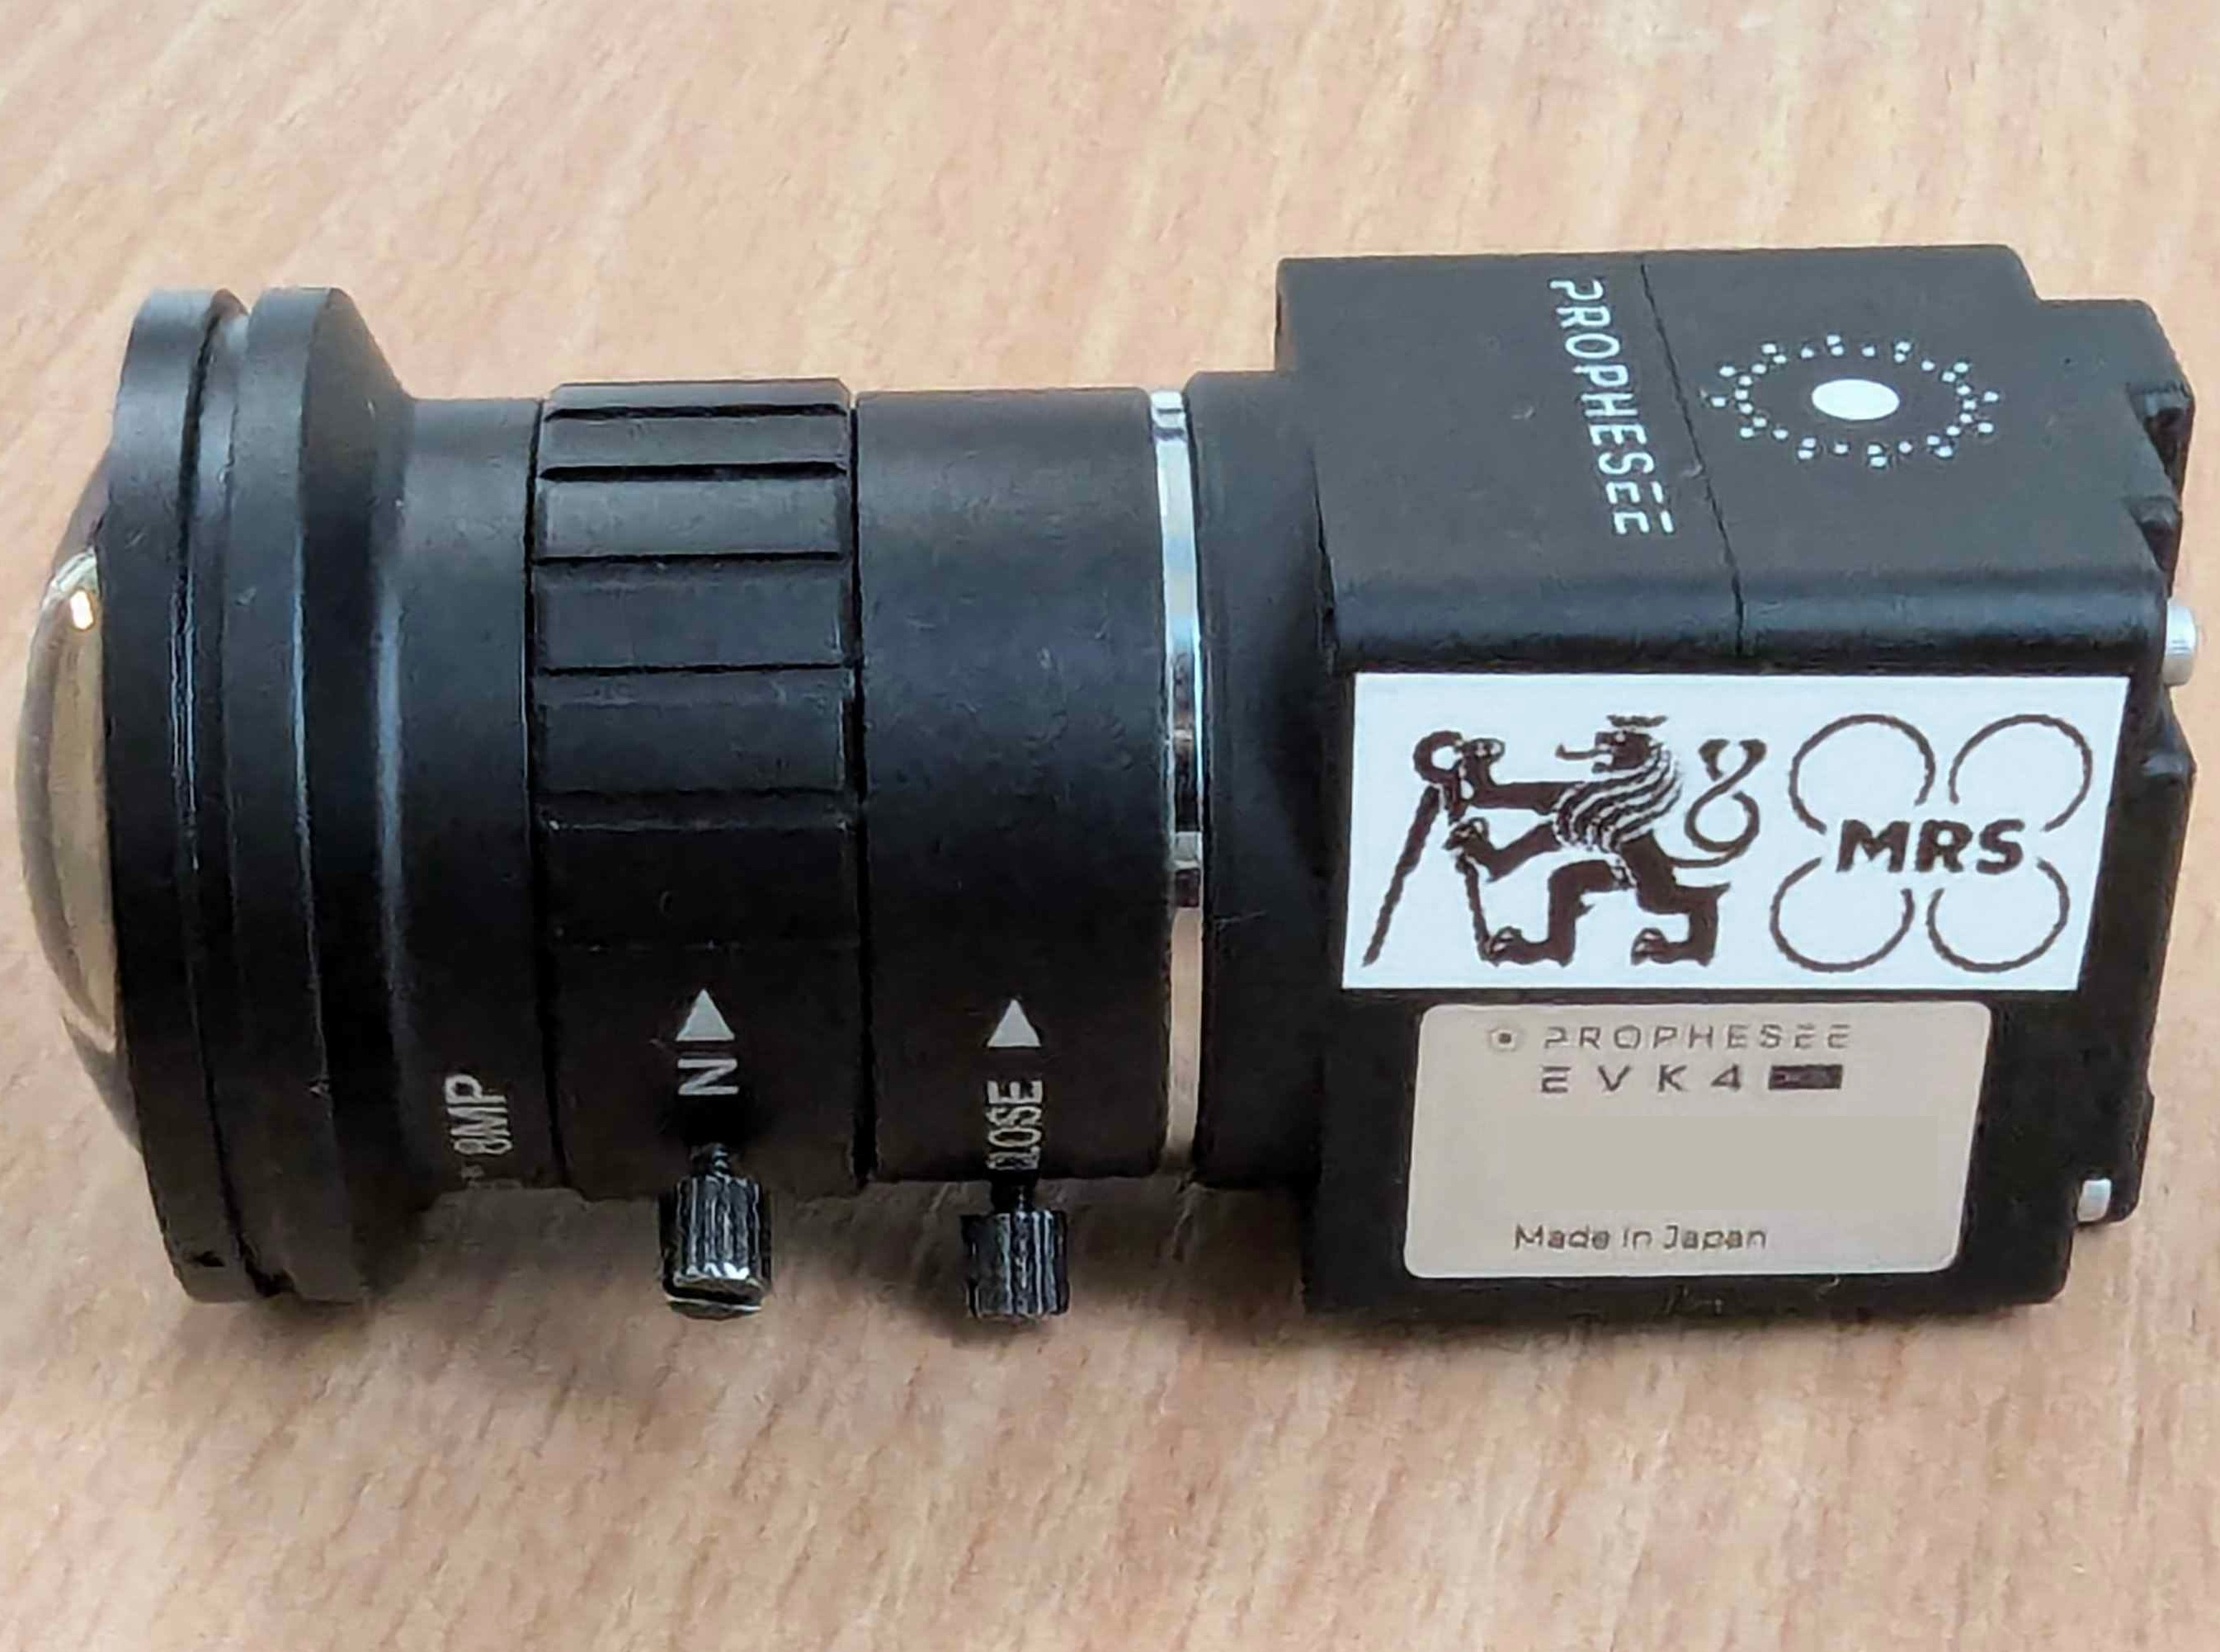
\includegraphics[width=0.50\textwidth]{./fig/photos/camera_with_lens.jpg}
	\caption{The event based camera EVK4 from Prophesee with a 2.5mm F1.6 fish eye lens.}
	\label{fig:evk4}
\end{figure}

The data from the camera has been obtained using the Metavision Studio software, which records the data in the .raw format.
Data is then later processed using various functions of the Metavision SDK\footnote{Metavision SDK Docs: \url{https://docs.prophesee.ai/stable/index.html}},
which has either C++ or Python API. In this work, the Python API has been used.

\section{Data collection}

The data has been collected on several occasions by measuring a stationary UAV which is a part of the MRS UVDAR system, that
uses UV \ac{LED} sources for localization and communication between individual UAVs. 
Each UAV is equipped with 8 UV LEDs, with 2 LEDs on each arm of the UAV. Each of the LEDs can be individually controlled
and can be set to various sequences of blinking (not only on/off).

\subsection{Initial measurements}

The initial measurements were done by securing the event camera on a tripod and placing the UAV at distances ranging from
$0.5$ to $2.5$ meters. The LEDs were set to blink at a frequency in range of $1$ Hz to $30$ kHz. No \ac{ROI} was set
and the whole image has been recorded during the testing.

This first experiment proved to be rather inefficient, as the LEDs need to be isolated from each other's influence, which
was not done properly at this time. This problem is solvable in the post processing, by filtering out the events
by using a ROI filter, but this proved rather inefficient (it is possible to filter the events by finding bounding boxes
that encapsulate light sources, but on a more complex scene this approach becomes relatively hard).
The other issue turned out to be the reflections of surrounding objects (as seen on \reffig{fig:meas1}), which caused
another source of unwanted events in the recording.

\begin{figure}[htbp]
  \centering
  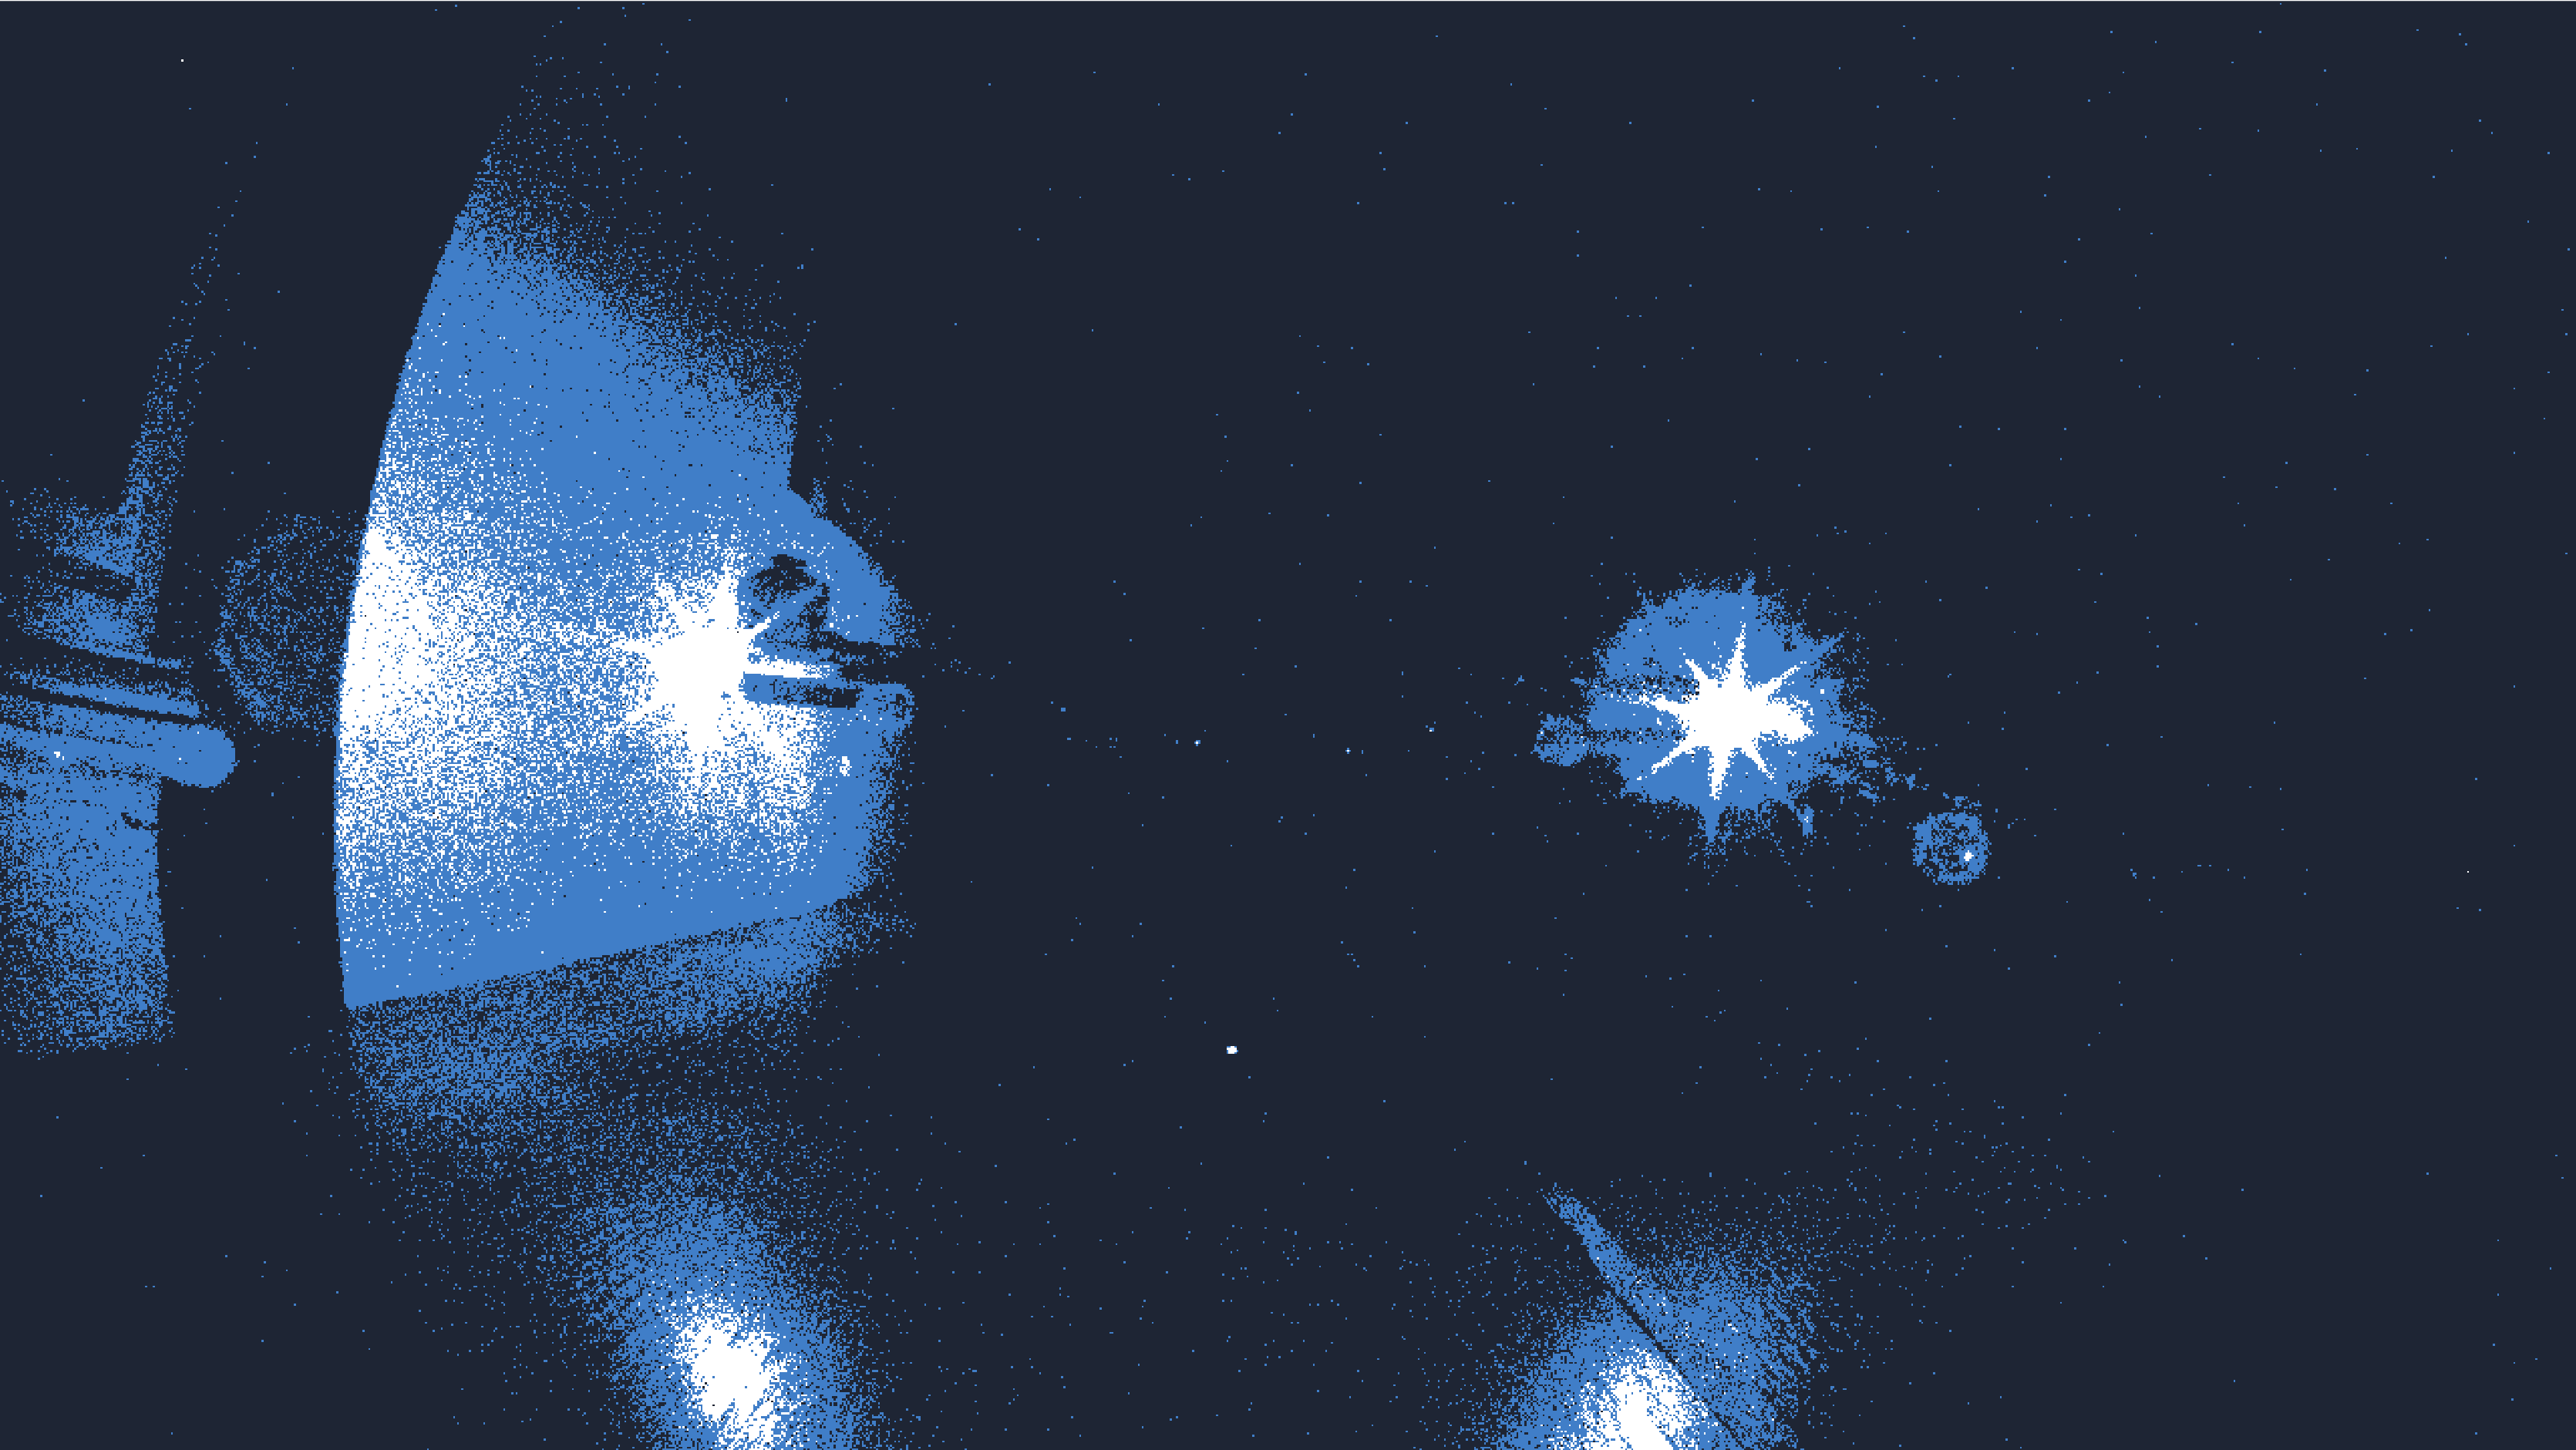
\includegraphics[width=0.5\textwidth]{./fig/photos/meas1.png}
  \caption{Visible reflections can be seen on the wall on the left side of the image.}
  \label{fig:meas1}
\end{figure}

\subsection{Distance - frequency influence}

In the following measurements, we consider one source of light as the whole arm of the UAV (with 2 UV LEDs). Measurements were
done on areas isolated by ROI filter directly in Metavision Studio - events were collected only on a select area, with the
rest of the events being discarded.
This time, the position of the UAV was fixed relative to the camera on a blank background. The camera was placed on a tripod
and moved by increments of $0.2$ meters, starting from $1$ meter and ending at $3$ meters, with additional measurements done
at $4$ and $5$ meters.

Frequency range of the LED modulation was set in a range from $10$ Hz to $30$ kHz.

\subsection{Rotation angle influence}

In addition to a distance and frequency influence, the rotation angle influence also needs to be considered, to
verify the emitting characteristics of the light sources - if they can or cannot be considered lambertian.
The UAV was rotated by increments of $45$ degrees relative to the event camera, at distances of $0.5$, $1$ and $2$ meters,
with frequencies ranging from $10$ Hz to $10$ kHz. 

\subsection{RSSR Data collection}

Another dataset will be collected for the application of \ac{RSSR} \cite{bai2021vlp},
which will serve as the focus of the subsequent bachelor thesis that builds upon this semester project.

%% --------------------------------------------------------------
%% |                The main section of the thesis              |
%% --------------------------------------------------------------

%!TEX root = ../main.tex

\chapter{Data processing\label{chap:data_processing}}

The data has ben analyzed using Python in a Jupyter notebook\footnote{Source code is available at: \url{https://github.com/kubakubakuba/mrs-uvdar-distance-estimator}}, with libraries from Metavision SDK.

\section{Distance - frequency influence}

The distance frequency dataset has recordings of the UAV placed at 0 and 45 degrees relative to the event camera. This ensures data is captured from either
one LED source pointed directly at the event camera, or 2 LED sources pointed at the event camera at an angle. At each distance a new subdirectory was
created, with its name being the distance in meters and the content being the recordings of various frequencies in sequence, ordered by the recording timetamp.

With the range of frequencies\footnote{The frequencies represented in this list are the actual frequencies sent to the UVDAR unit. The preserved frequencies
are half of the values in this list - UVDAR interprets the frequency with a reference to the length of the sequence (2 for on/off).} and distances being

\begin{lstlisting}
frequencies_Hz = [10, 25, 50, 100, 250, 500, 1000, 2500, 5000, 10000, 20000, 30000]
distances_m = [1.0, 1.2, 1.4, 1.6, 1.8, 2.0, 2.2, 2.4, 2.6, 2.8, 3.0, 4.0, 5.0]
\end{lstlisting}

We can load the dataset stored in raw files into a matrix representing the distances and frequencies, then load a select amount of events from each file.
The data is then resampled to a 1D array by summing polarities over a select bin width. Peaks in this signal are then analyzed by scipy's findpeaks function,
and the average amount of events with the standard deviation is calculated for each frequency and distance.

We can see the influence of distance and frequency on the average number of events on
\reffig{fig:dist} and \reffig{fig:freqs} respectively. If we fit a inverse square law function,
which can be expressed as
\begin{equation}
	\text{intensity} \propto \frac{1}{\text{distance}^2}
\end{equation}
to the data shown in \reffig{fig:fit1}, we can show that the inverse square law model
approximates the data reasonably well.
More complex functions could be used to fit the data, but it would rather tend to overfitting instead
of representing the data in a more general way.

\begin{figure}[htbp]
	\centering
	\subfloat[Influence of distance on the average number of events.] {
	  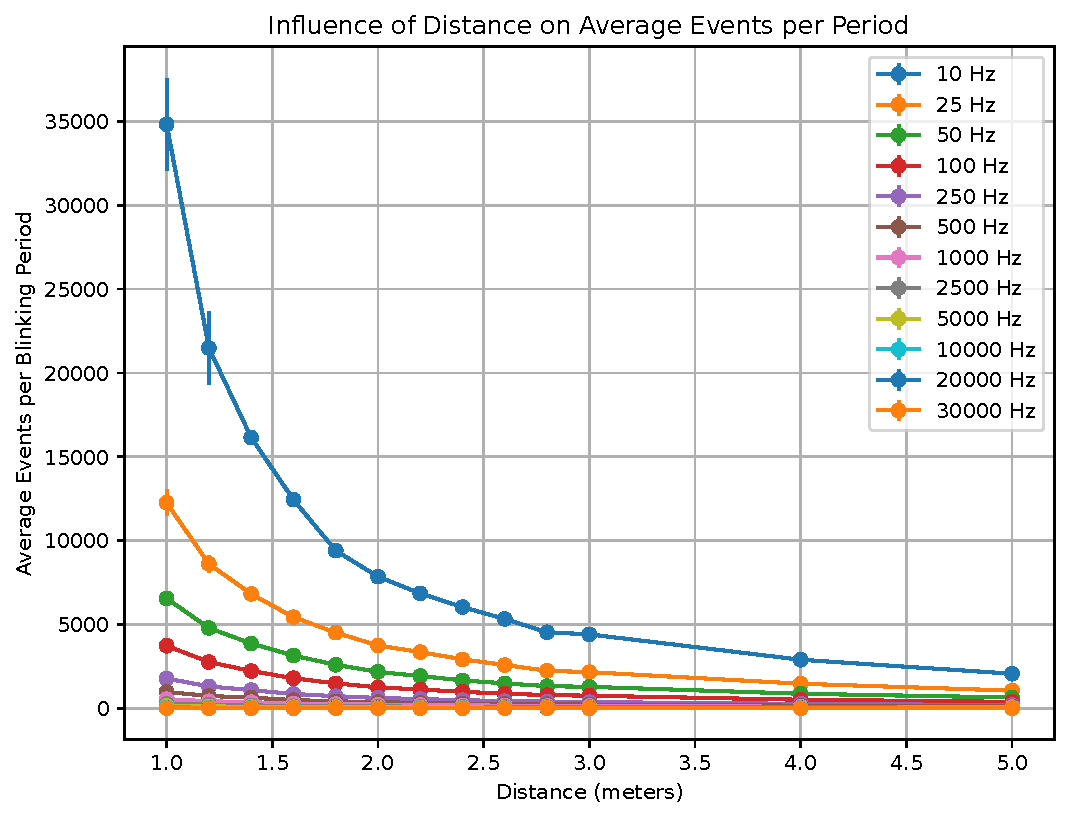
\includegraphics[width=0.5\textwidth]{./fig/plots/dist.pdf}
	  \label{fig:dist_1}
	}
	\subfloat[Influence of distance on the log of average number of events.] {
	  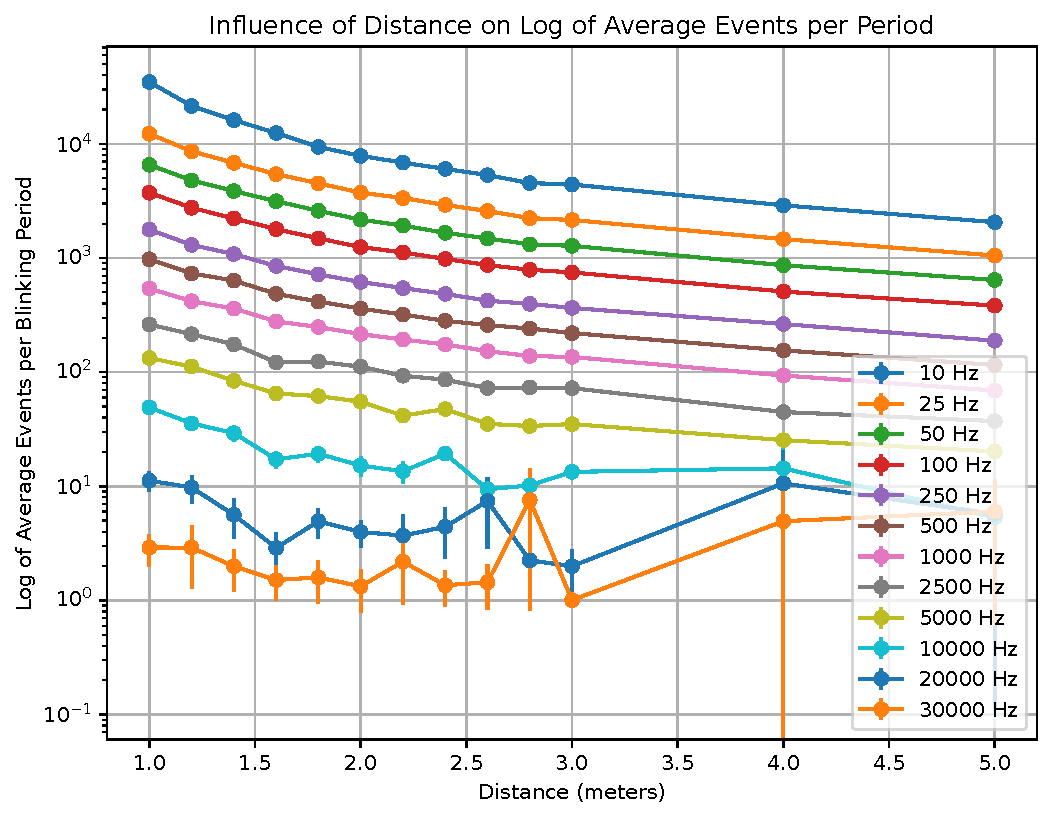
\includegraphics[width=0.5\textwidth]{./fig/plots/distlog.pdf}
	  \label{fig:dist_2}
	}
	\caption{
  The influence of distance on the average number of events with the UAV rotated 0 degrees relative to the event camera on \reffig{fig:dist_1}, and with the log of the average number of events on \reffig{fig:dist_2}.
  }
	\label{fig:dist}
\end{figure}

\begin{figure}[htbp]
	\centering
	\subfloat[Influence of frequency on the average number of events.] {
	  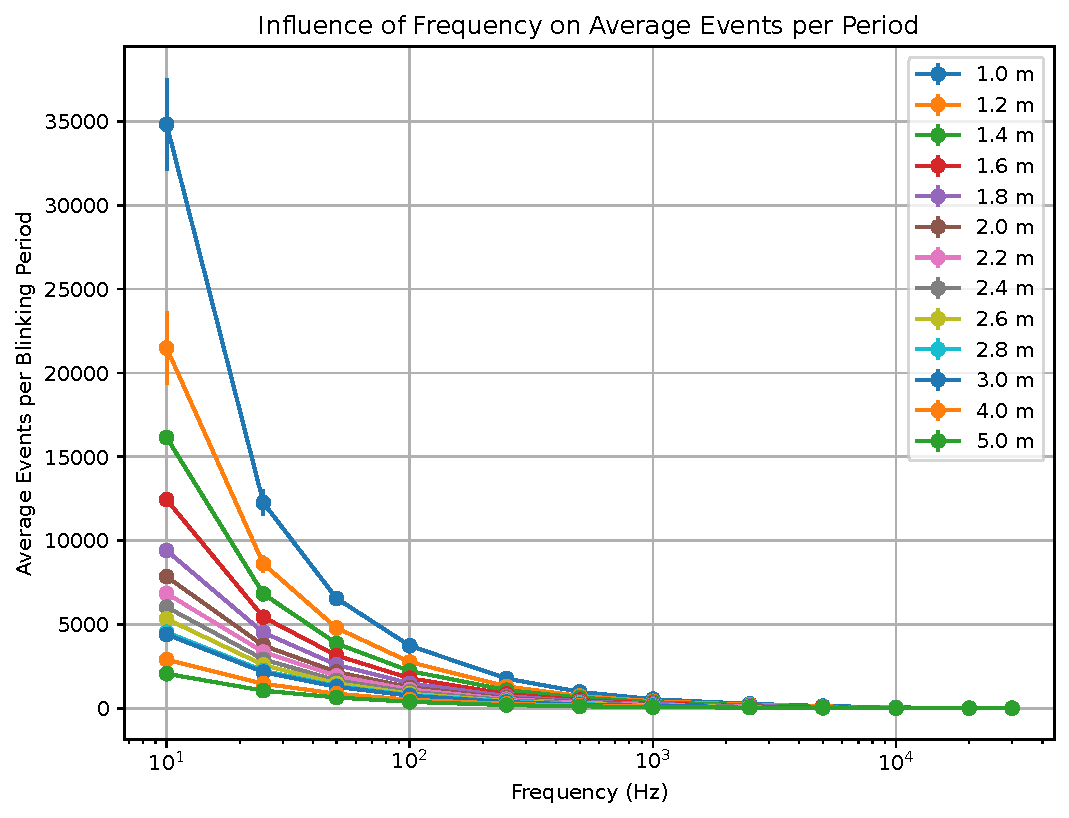
\includegraphics[width=0.5\textwidth]{./fig/plots/freqs.pdf}
	  \label{fig:freqs_1}
	}
	\subfloat[Influence of frequency on the log of average number of events.] {
	  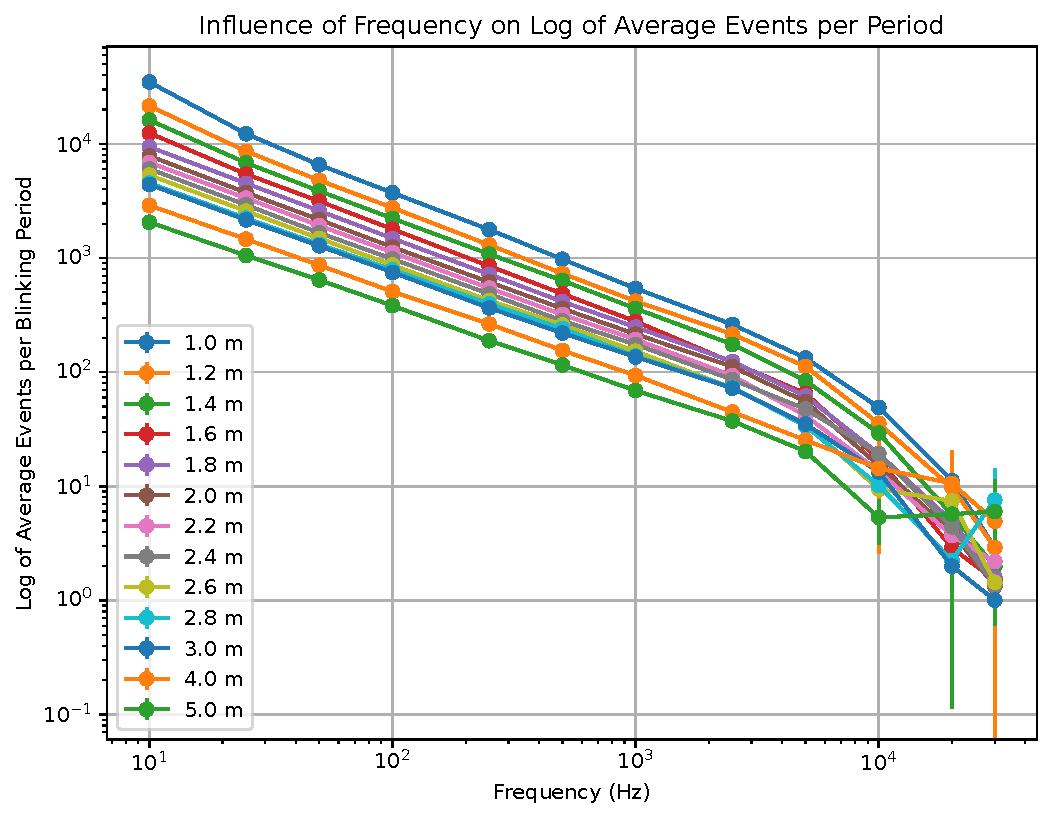
\includegraphics[width=0.5\textwidth]{./fig/plots/freqslog.pdf}
	  \label{fig:freqs_2}
	}
	\caption{
  The influence of frequency on the average number of events with the UAV rotated 0 degrees relative to the event camera on \reffig{fig:freqs_1}, and with the log of the average number of events on \reffig{fig:freqs_2}.
  }
	\label{fig:freqs}
\end{figure}

\begin{figure}[htbp]
	\centering
	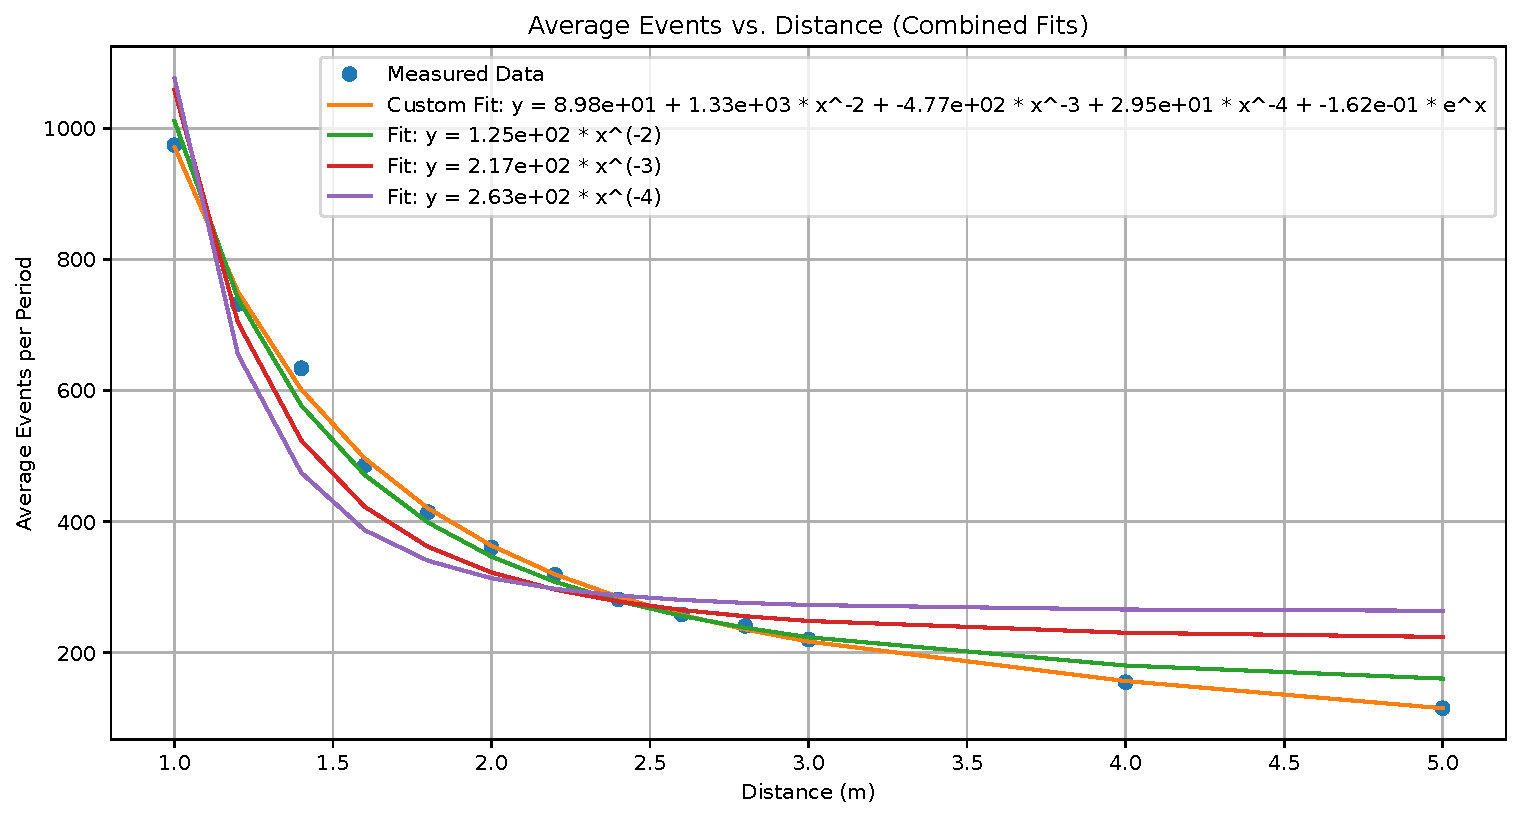
\includegraphics[width=0.90\textwidth]{./fig/plots/fit.pdf}
	\caption{Influence of distance data fitted with polynomial and exponential function.}
	\label{fig:fit1}
  \end{figure}

\newpage

\section{Rotation angle influence}

From the manufacturers datasheet for the UV LEDs\footnote{The datasheet of ProLight PM2B-1LLE 1W UV Power LED can be obtained from \url{https://www.tme.eu/Document/9dfb498784ffdd07892a42f4f17c6f37/PM2B-1LLE-DTE.pdf}}
used in the UVDAR system, we can learn that the LEDs have a lambertian radiation pattern,
which can be seen on \reffig{fig:lambertian}.

\begin {figure}[htbp]
	\centering
	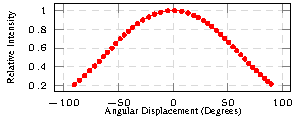
\includegraphics[width=0.75\textwidth]{./fig/plots/lambertian/lambertian.pdf}
	\caption{Lambertian radiation pattern of the UV LED.}
	\label{fig:lambertian}
\end{figure}

This means that the intensity of the light emmited from the LED decreases with the cosine
of the angle between the normal of the LED and the direction of the light \refeq{eq:lambertian}.

\begin{equation}
	I(\theta) = I_0\cos(\theta)
	\label{eq:lambertian}
\end{equation}

If we shift those distributions by $\pm 45$ degrees and sum them together, we can see the
theoretical distribution of the light emmited from the singular UAV arm \reffig{fig:lambert_combined}.
\begin {figure}[htbp]
	\centering
	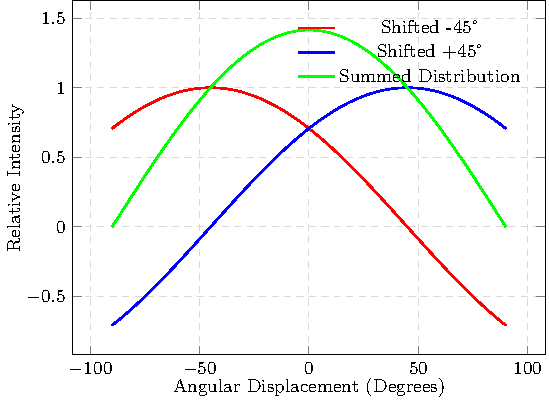
\includegraphics[width=0.75\textwidth]{./fig/plots/lambertian/3lambertian.pdf}
	\caption{Radiation pattern of two lambertian light sources shifted by $\pm 45$ degrees.}
	\label{fig:lambert_combined}
\end{figure}
With the dataset of the rotation of the UAV relative to the camera we will get the following results
on \reffig{fig:angles}.

\begin{figure}[htbp]
	\centering
	\subfloat[Influence of rotation of the UAV on the log of average number of events at 0.5 m.] {
	  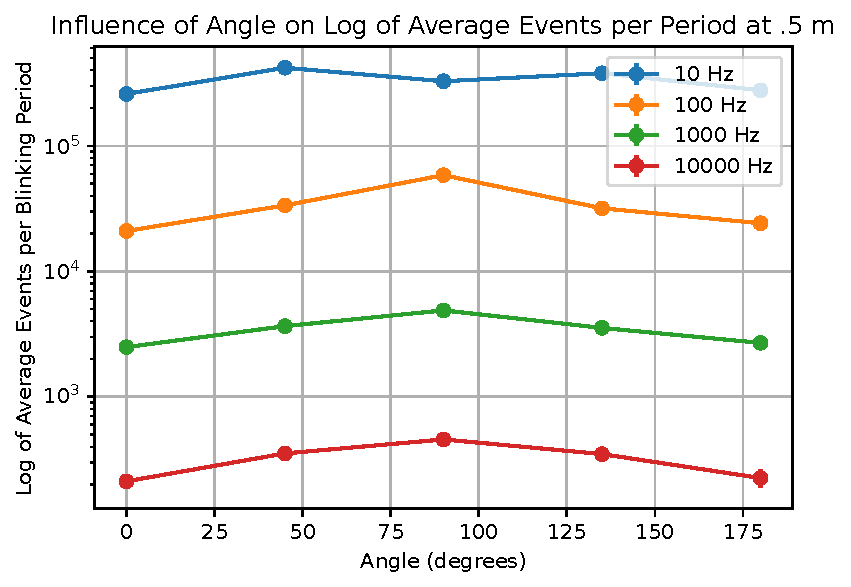
\includegraphics[width=0.5\textwidth]{./fig/plots/angle/angle1.pdf}
	  \label{fig:angle_1}
	}
	% \subfloat[Influence of rotation of the UAV on the log of average number of events at 1 m.] {
	%   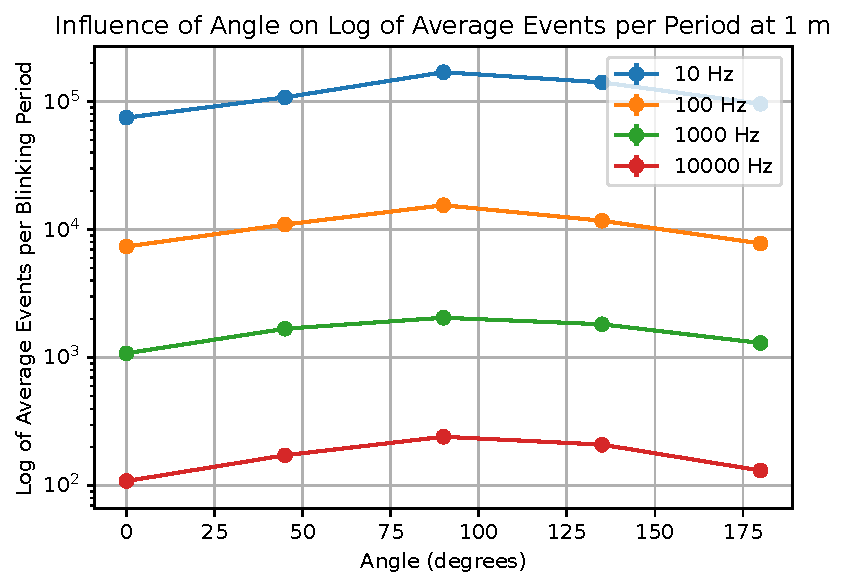
\includegraphics[width=0.5\textwidth]{./fig/plots/angle/angle2.pdf}
	%   \label{fig:angle_2}
	% }
	\subfloat[Influence of rotation of the UAV on the log of average number of events at 2 m.] {
	  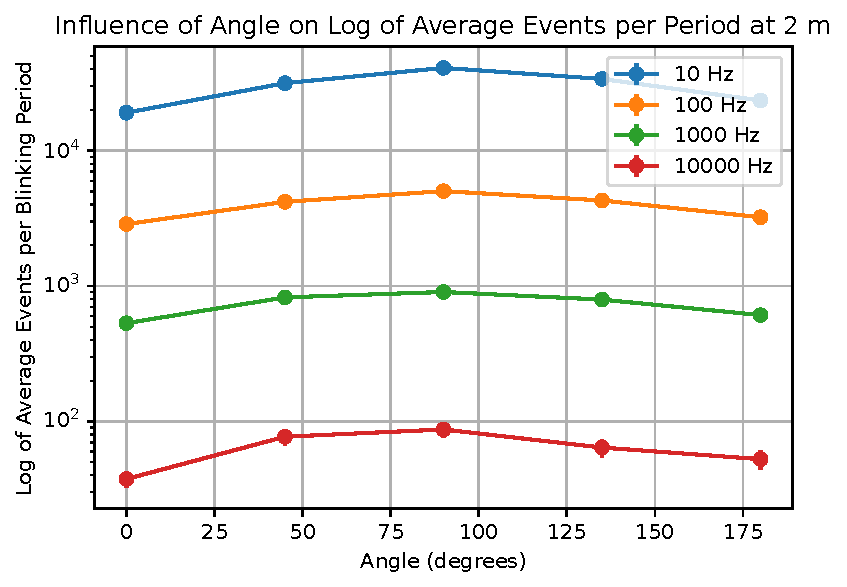
\includegraphics[width=0.5\textwidth]{./fig/plots/angle/angle3.pdf}
	  \label{fig:angle_3}
	}
	\caption{
  The influence of rotation angle on the log of average number of events at 0.5 m on \reffig{fig:angle_1} and at 2 m on \reffig{fig:angle_3}.
  }
	\label{fig:angles}
\end{figure}

The data shows a rough approximation of the theoretical distribution on \reffig{fig:lambert_combined},
but with a drop of intensity at the middle of the distribution. This could be caused
by the fact that the LEDs, when close to the camera, can be perceived as multiple sources,
but when moved further away, they merge into one source as shown on \reffig{fig:leds}.

\begin{figure}[htbp]
	\centering
	\subfloat[2 LEDs with blinking frequency of 10 Hz at 0.5 m.] {
	  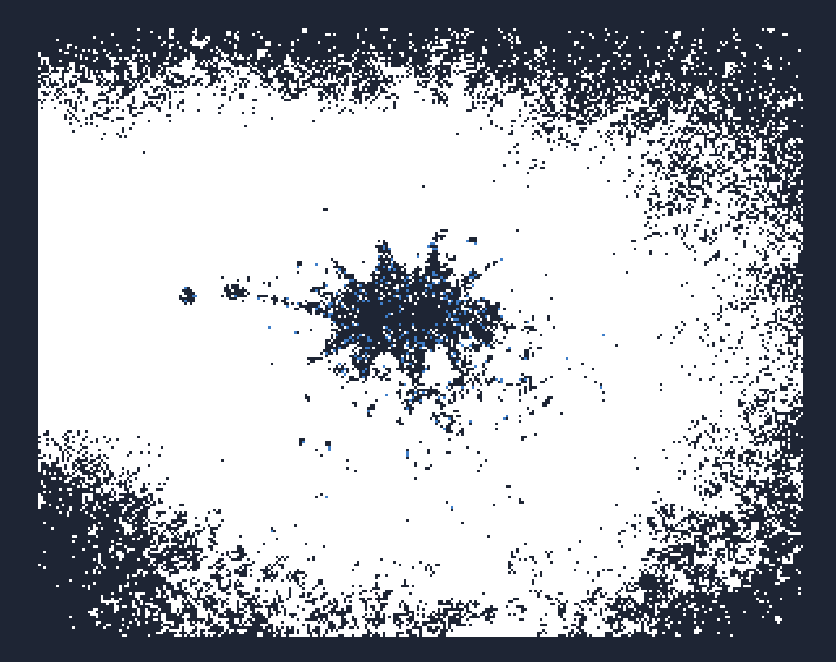
\includegraphics[width=0.5\textwidth]{./fig/photos/2leds_05m.png}
	  \label{fig:leds_1}
	}
	\subfloat[2 LEDs with blinking frequency of 10 Hz at 2 m.] {
	  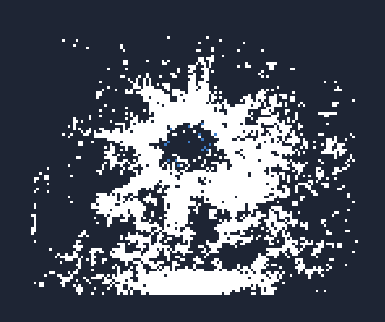
\includegraphics[width=0.5\textwidth]{./fig/photos/2leds_2m.png}
	  \label{fig:leds_2}
	}
	\caption{
  The light source on one arm of the UAV, consisting of two UV LEDs, blinking at a frequency of 10 Hz,
  placed at 0.5 m on \reffig{fig:leds_1} and 2 m at \reffig{fig:leds_2}. Star-like shape of
  the led source is caused by light diffraction that is happening when the intense
  monochromatic light enters the camera lens aperture.
  }
	\label{fig:leds}
\end{figure}

%% --------------------------------------------------------------
%% |                         Conclusion                         |
%% --------------------------------------------------------------

%!TEX root = ../main.tex

\chapter{Conclusion\label{chap:conclusion}}

This work has shown the influence of distance and frequency of modulated light sources on the response of an event based camera.
We have shown that the average number of events decreases with the increase of distance and can be approximated with
the inverse square law. The average number of events also decreases with the increase of frequency, as the camera is not
able to capture all the changes generated by the light source. What is also possible to observe from the results is the relatively
small distance range, in which the camera detects higher frequencies.

The influence of the rotation angle has also been examined, and has shown that the light source of each of the UAV arms can be
approximated with a lambertian emission model. Each of the arms can then be approximated as two lambertian sources, shifted
by $\pm 45$ degrees from the center of the arm. The real emission pattern approaches the theoretical model with the increase
of distance.

The RSSR method will be used in the subsequent bachelor thesis, where the UAV uses all of its 4 arms with different frequencies
to localize itself in the environment. This will be done by measuring the ratio of the received light intensity from each of the
arms. The camera will need to be calibrated using a calibrattion lattice of LEDs, the video data will need to be transformed
to get rid of the fish eye lens effect and to measure distances correctly.

%% --------------------------------------------------------------
%% |                         References                         |
%% --------------------------------------------------------------

\chapter{References}

\printbibliography[heading=none,title={}]

%% --------------------------------------------------------------
%% |                         Appendices                         |
%% --------------------------------------------------------------

% \appendix
% \renewcommand\chaptername{Appendix}

% \renewcommand{\thechapter}{A}
% \renewcommand\chaptername{Appendix A}

% \chapter{Appendix A}

%count the number of words

\end{document}
